\documentclass[12pt,fleqn]{article}\usepackage{../../common}
\begin{document}
Direkli Araba, Ters Sarka� (Cart Pole, Inverted Pendulum)

Sadece sa�a ve sola giden bir araba �zerinde duran bir direk var. Bu
dire�in �zerinde bir k�tle var; acaba bu dire�i sadece arabay� sa�a sola
g�t�rerek dengeleyebilir miyiz? Belki baz�lar�m�z elimiz �zerinde bir
sopay� dengelemeye u�ra�m���zd�r, yapmaya �al��aca��m�z buna �ok benziyor.  

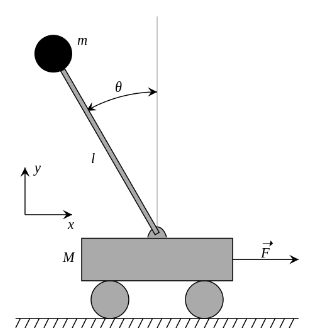
\includegraphics[width=15em]{phy_cartpole_01.png}

Sistemin hareket denklemlerini modellemek icin Lagrange formullerini
kullanacagiz. $L = K - P$ uzerinden,

$$
L = \frac{1}{2} M v_1^2 + \frac{1}{2} m v_2^2 - m g \ell \cos\theta
$$












2.160 pdf sf 75 algebr ricc


\end{document}

















